\justifying
\noindent

\section{Introduction}

With the availability of increased processing power and memory of personal computers, today Computer Numerical Control (CNC) interpolation is mostly carried out using computer software instead of electronic hardware devices with mathematical logic, for example, the Digital Differential Analyser (DDA) integrator. The basic theory and design of CNC systems, however, have remain the same since its beginning \cite{SuhBook_2008}. 
\vspace*{1\baselineskip}


The two common types of CNC software interpolation techniques are Reference-Pulse Interpolation \cite{Giap_2014},\cite{Koren_1981}, and Reference-Word (Sampled-Data) Interpolation \cite{Koren_1982}, \cite{Koren_1978}. 

	%% NOT VISIBLE
	\index{Reference-Pulse interpolation}
	\index{Reference-Word interpolation} 
	\index{Sampled-Data interpolation}
	\vspace*{1\baselineskip}

Over time, various algorithms have been proposed for CNC software interpolation. For example, techniques for Reference-Pulse interpolation include software version of the Digital Differential Analyser (SDDA), the Stairs Approximation and the Direct Search Interpolation. 

	%% NOT VISIBLE
	\index{Digital Differential Analyser} 
	\index{Stairs Approximation interpolation} 
	\index{Direct Search interpolation}
	\vspace*{1\baselineskip}

Techniques for Reference-Word interpolation include Euler, Improved Euler, Taylor, Tustin and Improved Tustin interpolations.

	%% NOT VISIBLE
	\index{Euler interpolation}
	\index{Improved Euler interpolation}
	\index{Taylor interpolation}
	\index{Tustin interpolation}
	\index{Improved Tustin interpolation}
	\vspace*{1\baselineskip}

In CNC machine operation, the function of interpolation is to generate coordinated movements to drive the separate axis-of-motions and/or rotation axes in order to achieve the desired path of the CNC cutting or milling tool relative to the workpiece. Essentially, interpolation generates the final reference commands that moves stepper or servo motor drives to produce the physical part that is to be machined. Reference commands mean commands to the CNC tool to trace/follow (refer to) the desired path or trajectory.

%% NOT VISIBLE
	\index{Milling tool}
	\index{Reference command}

% =====================================
\section{Types of CNC Machines}
%======================================

There are various types of CNC machines. The main categories are CNC Milling, CNC Lathe, CNC Router and CNC 3D Printing machines. There are many sub-categories, covering variations of CNC machines, and it is too numerous to list. 
\vspace*{1\baselineskip}

These machines share one common characteristic, that is, they all are numerically controlled by a computer, thus adopting the name Computer Numerical Control (CNC) machines. Most CNC machines cut or remove materials in order to produce a machined part. The exception is the CNC 3D Printing machine where materials are instead deposited layer by layer to produce a part.

\subsection{CNC Milling Machine}

CNC milling devices are the most widely used type of CNC machine. It is a machine that produces a work part by both drilling and cutting using a rotating cylindrical cutting tool. In a milling machine, the cutter is able to move along multiple axes simultaneously. It can create a part with a variety of shapes, slots and holes. To produce a part, the work-piece in a milling machine is often moved across the milling tool (drill cutter) in different directions, like linear table movements and circular table rotations.  Common milling machines offer from 3 to 5 motion axes. Please see Fig. ~\ref{fig:App1-CNC-Milling-Machine.jpg}, a link to the image of a typical CNC Milling machine.

\subsection{CNC Lathe Machine}

The CNC lathe machine is a machine that rotates a workpiece on a spindle to cut away excess material. The lathe uses cutting tools and drill bits with different diameters to apply on the workpiece and produce a symmetrical object. In a lathe machine, the cutter is not able to move along multiple axes. These machines can produce objects in a variety of shapes, cuts, and details based on cutting a rotating work piece. The two lathe configuration types are the CNC horizontal lathe and the CNC vertical lathe. Please see Fig. ~\ref{fig:App1-CNC-Lathe-Machine.jpg}, a link to the image of a typical CNC Lathe machine.

\subsection{CNC Router Machine}

The CNC router machine is very similar in concept to a CNC milling machine. Instead of routing by hand, tool paths for the CNC router are controlled via computer numerical control system. The word rout means to "hollow out" an area in relatively hard material. Routers are normally used for cutting various hard materials, such as engraving wood, composites, aluminum, steel, ceramics, plastics, glass, and foams. The application of routers are mainly in woodworking, especially building cabinets,  engraving decorations, doors or panels. Routers are not generally used for drilling or 3D model machining. Please see Fig. ~\ref{fig:App1-CNC-Routing-Machine.jpg}, a link to the image of a typical CNC Routing machine.

\subsection{CNC 3D Printing}

The CNC 3D Printing machine is a machine in which material is deposited, joined or solidified under computer control to create a three-dimensional object. Many different technologies are used in the 3D printing process, the most common being the fused deposit modeling (FDM) method. The machine uses inkjet-technology nozzles to apply a specialized thick liquid or powder to form each new layer. Common materials used in 3D printing are thick waxes and plastic polymers. 
Please see Fig. ~\ref{fig:App1-CNC-3D-Printing-Machine.jpg}, a link to the image of a typical CNC 3D Printing machine.

%% =================================
\subsection{Recent Designs in CNC Systems}

On designs in CNC machine architectures, recent developments in CNC systems include, for example, designs with the introduction of more motion axes (up to 9 axes), cutting under water or fluid immersion environments, new sensors, smart computing, high-speed machining, energy efficient techniques, artificial intelligence control, wastage reduction in materials removal, process monitoring, machining management operations, modular software construction, and human-machine interface. 
\vspace*{1\baselineskip}

On designs in CNC machining control, new developments include design, for example, in software algorithms and methods, for path motion smoothness, for machining speed control, for addressing acceleration and deceleration effects, for 2D path error reduction, for 3D contouring error control, for compensating tool jerks, vibrations, heating and friction effects.         


\pagebreak
\clearpage
% ==========================================
\section{Basic architecture of a typical CNC system} 

\begin{figure}[htbp]
	\begin{center}
		\frame{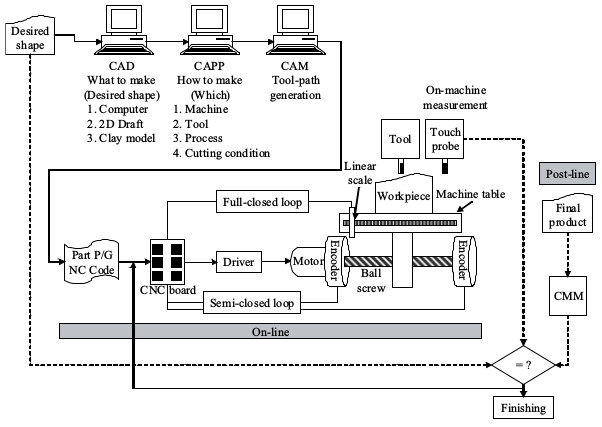
\includegraphics[width=0.95\textwidth]{./07-images/img-Ch1/CNC-Basic-Architecture.jpg}}
		\caption{Basic architecture of a typical CNC system.}
		\label{fig:CNC-Basic-Architecture.jpg}
	\end{center}
\end{figure}

\begin{figure}[htbp]
	\begin{center}
		\frame{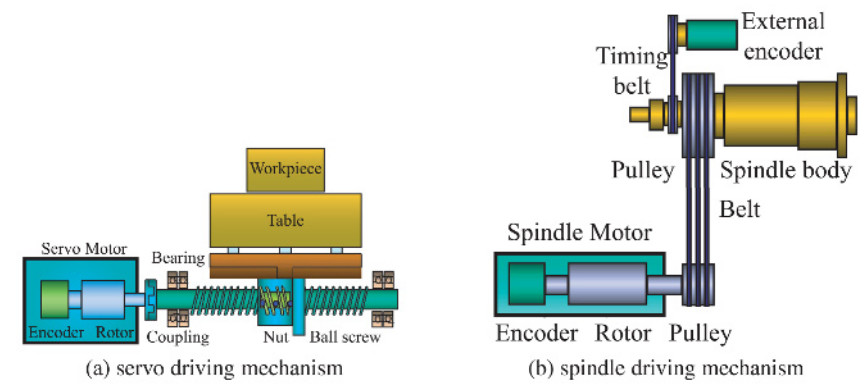
\includegraphics[width=0.68\textwidth]{./07-images/img-Ch1/CNC-Servo-and-Spindle-Driving-Mechanism.jpg}}
		\caption{CNC Servo and Spindle Driving Mechanism}
		\label{fig:CNC-Servo-and-Spindle-Driving-Mechanism.jpg}
	\end{center}
\end{figure}


\pagebreak
\clearpage
% ==========================================
\section{Process Flow for a typical CNC system}

\begin{figure}[htbp]
	\begin{center}
		\frame{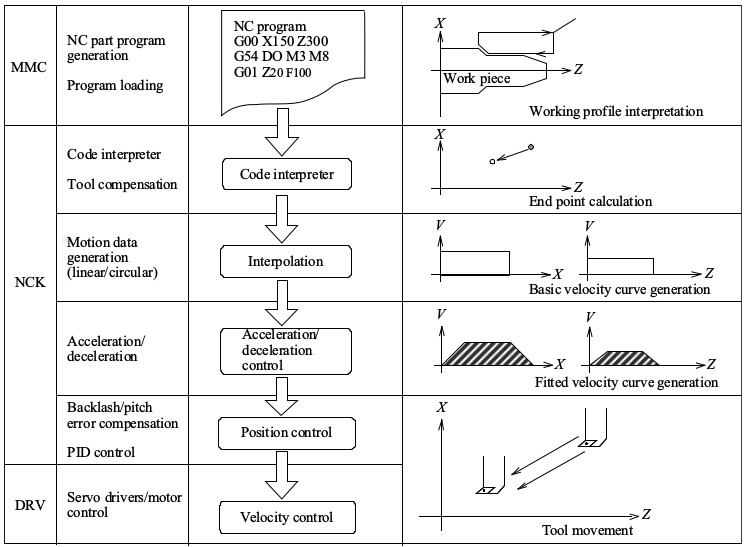
\includegraphics[width=0.98\textwidth]{./07-images/img-Ch1/CNC-Typical-Software-Control-Flow-Diagram.jpg}}
		\caption{Process Flow for a typical CNC system}
		\label{fig:CNC-Typical-Software-Control-Flow-Diagram.jpg}
	\end{center}
\end{figure}

Legend\\
\begin{enumerate}
	\item MMC Man-Machine Control
	\item NCK Numerical Control Kernel
	\item DRV Driver Module
	\item NC  Numerical Control
	\item PID Proportional Integrative Derivative
\end{enumerate}


\pagebreak
\clearpage
% ==========================================
\section{Functional block diagram for a typical CNC system} 

CNC manufacturing operations involve the generation of reference signals describing the geometrical parts to be machined and the control of the machine. The control is such that it follows those reference signals. In modern CNC machines, the generation of reference signals, construction and execution of control loops are accomplished in software within a computer.    
\vspace*{1\baselineskip}

The figure below shows the functional block diagram for a typical CNC system. The meanings of terms used are described in Table [~\ref{table:CNC-Terminology Part 1 of 2}] and Table [~\ref{table:CNC-Terminology Part 2 of 2}]. 

\begin{figure}[htbp]
	\begin{center}
		\frame{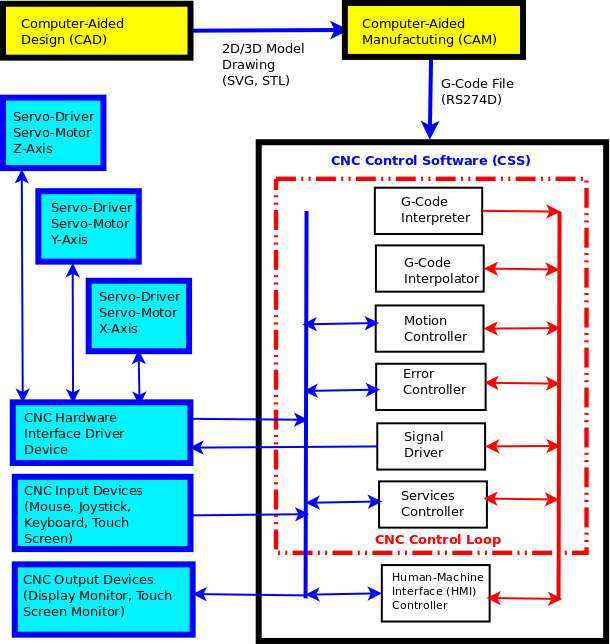
\includegraphics[width=0.95\textwidth]{./06-diagrams/dia-Ch1/Components-of-CNC-System.jpg}}
		\caption{Functional Block Diagram for CNC system}
		\label{fig:Functional-Block-Diagram-for-CNC-System.jpg}
	\end{center}
\end{figure}

% =========================================
%%\clearpage
%%\pagebreak

%% \section{Process flow chart for a typical CNC system}

%% YES. tikz package working
%%% =========================================================
% % % =========================================================
% % % =========================================================
% % \input{./diagrams/dia-Ch1/test-tikz.tex}
% =========================================================

%% TikZ is a very large program which can do lots of things. You will find commands to draw hierarchial trees, to draw lots of different types of shapes, to do some elementary programming, to align elements of a picture in a matrix frame, to decorate nodes, to compute the intersections of paths, etc.  The main message is “if it is not in these notes, it is most probably somewhere in the manual”


\begin{center}
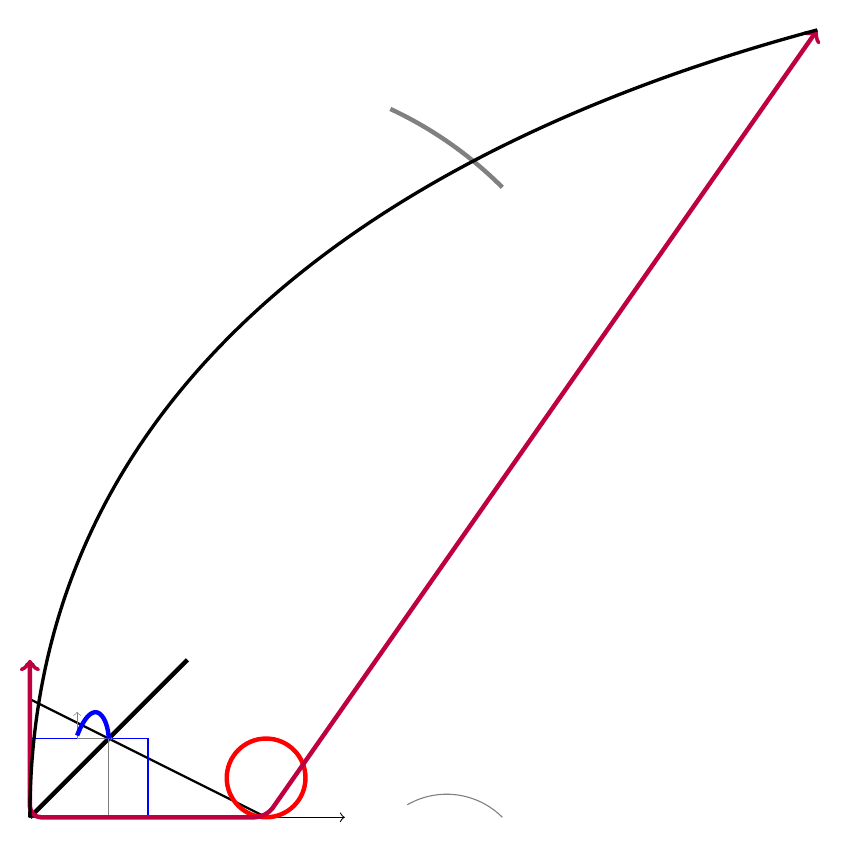
\begin{tikzpicture}

\draw [<->] (0,2) -- (0,0) -- (4,0);
\draw [thick] (0,1.5) -- (3,0);
\draw [ultra thick] (0,0) -- (2,2);
\draw [help lines] (1,0) -- (1,1) -- (0,1);

\draw [blue] (0,0) rectangle (1.5,1);
\draw [red, ultra thick] (3,0.5) circle [radius=0.5];;
\draw [gray] (6,0) arc [radius=1, start angle=45, end angle= 120];


\draw [<->, rounded corners, ultra thick, purple] (0,2) -- (0,0) -- (3,0) -- (10, 10);


\draw [gray, ultra thick] (6,8) arc [radius=5, start angle=45, end angle= 65];

\draw[very thick] (0,0) to [out=90,in=195] (10,10);

\draw [<->, help lines] (0.6,1.34) -- (0.6,1) -- (1.05,1);
\draw[blue, ultra thick] (0.6, 1.0385) -- (0.61, 1.06372) -- (0.62, 1.08756) -- (0.63, 1.11012) -- (0.64,1.13147) -- (0.65, 1.15166) -- (0.66, 1.17074) -- (0.67, 1.18874) -- (0.68,1.20568) -- (0.69, 1.22157) -- (0.7, 1.23643) -- (0.71, 1.25026) -- (0.72,1.26307) -- (0.73, 1.27486) -- (0.74, 1.28561) -- (0.75, 1.29534) -- (0.76, 1.30402) -- (0.77, 1.31165) -- (0.78, 1.31821) -- (0.79, 1.32369) -- (0.8, 1.32806) -- (0.81, 1.33131) -- (0.82, 1.3334) -- (0.83, 1.33431) -- (0.84, 1.334) -- (0.85, 1.33244) -- (0.86, 1.32956) -- (0.87, 1.32533) -- (0.88, 1.31966) -- (0.89, 1.3125) -- (0.9, 1.30373) -- (0.91, 1.29325) -- (0.92, 1.2809) -- (0.93, 1.26649) -- (0.94, 1.24976) -- (0.95, 1.23032) -- (0.96, 1.2076) -- (0.97, 1.18065) -- (0.98, 1.14763) -- (0.99, 1.1038) -- (0.991, 1.09836) -- (0.992, 1.09261) -- (0.993, 1.0865) -- (0.994, 1.07994) -- (0.995, 1.07282) -- (0.996, 1.06497) -- (0.997, 1.0561) -- (0.998, 1.04563) -- (0.999, 1.03209) -- (0.9991, 1.03042) -- (0.9992, 1.02866) -- (0.9993, 1.02679) -- (0.9994, 1.02478) -- (0.9995, 1.0226) -- (0.9996, 1.02019) -- (0.9997, 1.01747) -- (0.9998, 1.01424) -- (0.9999, 1.01005) -- (0.9999, 1.01005) -- (0.99991, 1.00953) -- (0.99992, 1.00898) -- (0.99993, 1.0084) -- (0.99994, 1.00778) -- (0.99995, 1.0071) -- (0.99996, 1.00634) -- (0.99997, 1.00549) -- (0.99998, 1.00448) -- (0.99999, 1.00317) -- (1,1);
\end{tikzpicture}
\end{center}


\begin{center}
\begin{tikzpicture}[domain=0:0.5,xscale=10,yscale=10]

\draw[<->] (0,2) node[left]{EUR}-- (0,0) -- (.7,0) node[below] {$q$};
\draw[red] plot (\x, {0.25+\x/2+\x*\x/2}) node[right] {$v_1(x)$};
\draw[green] plot (\x, {0.025+\x+\x*\x}) node[right] {$v_2(x)$};
\draw[thin, dashed] plot (\x, {0.275+1.5*\x+1.5*\x*\x}) ;
\draw[thick,domain=0:0.33666] plot (\x, {0.05+2*\x+2*\x*\x}) ;
\draw[thick,domain=0.33666:0.5]
plot (\x, {0.5+\x+\x*\x}) node[right] {$2\min[v_1,v_2]$};


\end{tikzpicture}
\end{center}

% =========================================================

%% TikZ is a very large program which can do lots of things. You will find commands to draw hierarchial trees, to draw lots of different types of shapes, to do some elementary programming, to align elements of a picture in a matrix frame, to decorate nodes, to compute the intersections of paths, etc.  The main message is “if it is not in these notes, it is most probably somewhere in the manual”


\begin{center}
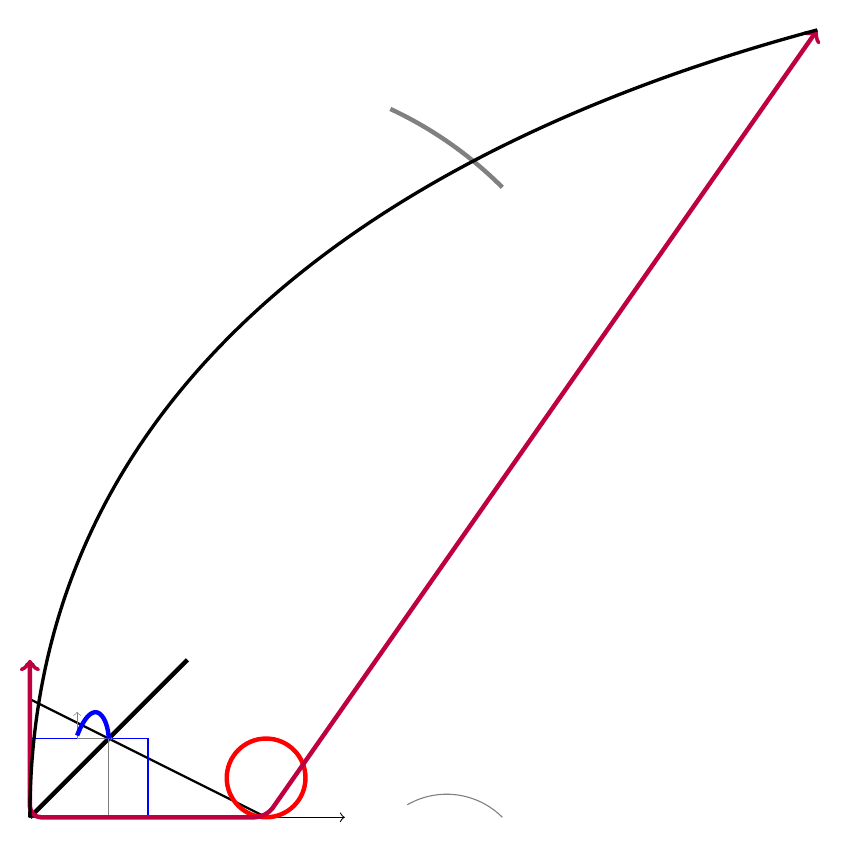
\begin{tikzpicture}

\draw [<->] (0,2) -- (0,0) -- (4,0);
\draw [thick] (0,1.5) -- (3,0);
\draw [ultra thick] (0,0) -- (2,2);
\draw [help lines] (1,0) -- (1,1) -- (0,1);

\draw [blue] (0,0) rectangle (1.5,1);
\draw [red, ultra thick] (3,0.5) circle [radius=0.5];;
\draw [gray] (6,0) arc [radius=1, start angle=45, end angle= 120];


\draw [<->, rounded corners, ultra thick, purple] (0,2) -- (0,0) -- (3,0) -- (10, 10);


\draw [gray, ultra thick] (6,8) arc [radius=5, start angle=45, end angle= 65];

\draw[very thick] (0,0) to [out=90,in=195] (10,10);

\draw [<->, help lines] (0.6,1.34) -- (0.6,1) -- (1.05,1);
\draw[blue, ultra thick] (0.6, 1.0385) -- (0.61, 1.06372) -- (0.62, 1.08756) -- (0.63, 1.11012) -- (0.64,1.13147) -- (0.65, 1.15166) -- (0.66, 1.17074) -- (0.67, 1.18874) -- (0.68,1.20568) -- (0.69, 1.22157) -- (0.7, 1.23643) -- (0.71, 1.25026) -- (0.72,1.26307) -- (0.73, 1.27486) -- (0.74, 1.28561) -- (0.75, 1.29534) -- (0.76, 1.30402) -- (0.77, 1.31165) -- (0.78, 1.31821) -- (0.79, 1.32369) -- (0.8, 1.32806) -- (0.81, 1.33131) -- (0.82, 1.3334) -- (0.83, 1.33431) -- (0.84, 1.334) -- (0.85, 1.33244) -- (0.86, 1.32956) -- (0.87, 1.32533) -- (0.88, 1.31966) -- (0.89, 1.3125) -- (0.9, 1.30373) -- (0.91, 1.29325) -- (0.92, 1.2809) -- (0.93, 1.26649) -- (0.94, 1.24976) -- (0.95, 1.23032) -- (0.96, 1.2076) -- (0.97, 1.18065) -- (0.98, 1.14763) -- (0.99, 1.1038) -- (0.991, 1.09836) -- (0.992, 1.09261) -- (0.993, 1.0865) -- (0.994, 1.07994) -- (0.995, 1.07282) -- (0.996, 1.06497) -- (0.997, 1.0561) -- (0.998, 1.04563) -- (0.999, 1.03209) -- (0.9991, 1.03042) -- (0.9992, 1.02866) -- (0.9993, 1.02679) -- (0.9994, 1.02478) -- (0.9995, 1.0226) -- (0.9996, 1.02019) -- (0.9997, 1.01747) -- (0.9998, 1.01424) -- (0.9999, 1.01005) -- (0.9999, 1.01005) -- (0.99991, 1.00953) -- (0.99992, 1.00898) -- (0.99993, 1.0084) -- (0.99994, 1.00778) -- (0.99995, 1.0071) -- (0.99996, 1.00634) -- (0.99997, 1.00549) -- (0.99998, 1.00448) -- (0.99999, 1.00317) -- (1,1);
\end{tikzpicture}
\end{center}


\begin{center}
\begin{tikzpicture}[domain=0:0.5,xscale=10,yscale=10]

\draw[<->] (0,2) node[left]{EUR}-- (0,0) -- (.7,0) node[below] {$q$};
\draw[red] plot (\x, {0.25+\x/2+\x*\x/2}) node[right] {$v_1(x)$};
\draw[green] plot (\x, {0.025+\x+\x*\x}) node[right] {$v_2(x)$};
\draw[thin, dashed] plot (\x, {0.275+1.5*\x+1.5*\x*\x}) ;
\draw[thick,domain=0:0.33666] plot (\x, {0.05+2*\x+2*\x*\x}) ;
\draw[thick,domain=0.33666:0.5]
plot (\x, {0.5+\x+\x*\x}) node[right] {$2\min[v_1,v_2]$};


\end{tikzpicture}
\end{center}

% =========================================================

%% TikZ is a very large program which can do lots of things. You will find commands to draw hierarchial trees, to draw lots of different types of shapes, to do some elementary programming, to align elements of a picture in a matrix frame, to decorate nodes, to compute the intersections of paths, etc.  The main message is “if it is not in these notes, it is most probably somewhere in the manual”


\begin{center}
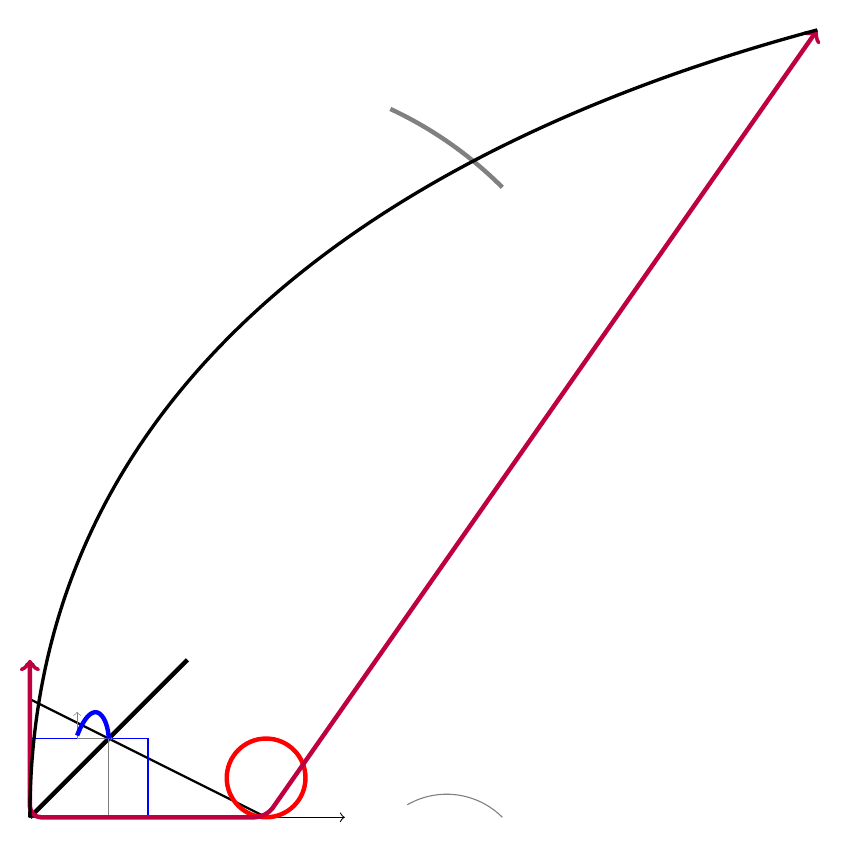
\begin{tikzpicture}

\draw [<->] (0,2) -- (0,0) -- (4,0);
\draw [thick] (0,1.5) -- (3,0);
\draw [ultra thick] (0,0) -- (2,2);
\draw [help lines] (1,0) -- (1,1) -- (0,1);

\draw [blue] (0,0) rectangle (1.5,1);
\draw [red, ultra thick] (3,0.5) circle [radius=0.5];;
\draw [gray] (6,0) arc [radius=1, start angle=45, end angle= 120];


\draw [<->, rounded corners, ultra thick, purple] (0,2) -- (0,0) -- (3,0) -- (10, 10);


\draw [gray, ultra thick] (6,8) arc [radius=5, start angle=45, end angle= 65];

\draw[very thick] (0,0) to [out=90,in=195] (10,10);

\draw [<->, help lines] (0.6,1.34) -- (0.6,1) -- (1.05,1);
\draw[blue, ultra thick] (0.6, 1.0385) -- (0.61, 1.06372) -- (0.62, 1.08756) -- (0.63, 1.11012) -- (0.64,1.13147) -- (0.65, 1.15166) -- (0.66, 1.17074) -- (0.67, 1.18874) -- (0.68,1.20568) -- (0.69, 1.22157) -- (0.7, 1.23643) -- (0.71, 1.25026) -- (0.72,1.26307) -- (0.73, 1.27486) -- (0.74, 1.28561) -- (0.75, 1.29534) -- (0.76, 1.30402) -- (0.77, 1.31165) -- (0.78, 1.31821) -- (0.79, 1.32369) -- (0.8, 1.32806) -- (0.81, 1.33131) -- (0.82, 1.3334) -- (0.83, 1.33431) -- (0.84, 1.334) -- (0.85, 1.33244) -- (0.86, 1.32956) -- (0.87, 1.32533) -- (0.88, 1.31966) -- (0.89, 1.3125) -- (0.9, 1.30373) -- (0.91, 1.29325) -- (0.92, 1.2809) -- (0.93, 1.26649) -- (0.94, 1.24976) -- (0.95, 1.23032) -- (0.96, 1.2076) -- (0.97, 1.18065) -- (0.98, 1.14763) -- (0.99, 1.1038) -- (0.991, 1.09836) -- (0.992, 1.09261) -- (0.993, 1.0865) -- (0.994, 1.07994) -- (0.995, 1.07282) -- (0.996, 1.06497) -- (0.997, 1.0561) -- (0.998, 1.04563) -- (0.999, 1.03209) -- (0.9991, 1.03042) -- (0.9992, 1.02866) -- (0.9993, 1.02679) -- (0.9994, 1.02478) -- (0.9995, 1.0226) -- (0.9996, 1.02019) -- (0.9997, 1.01747) -- (0.9998, 1.01424) -- (0.9999, 1.01005) -- (0.9999, 1.01005) -- (0.99991, 1.00953) -- (0.99992, 1.00898) -- (0.99993, 1.0084) -- (0.99994, 1.00778) -- (0.99995, 1.0071) -- (0.99996, 1.00634) -- (0.99997, 1.00549) -- (0.99998, 1.00448) -- (0.99999, 1.00317) -- (1,1);
\end{tikzpicture}
\end{center}


\begin{center}
\begin{tikzpicture}[domain=0:0.5,xscale=10,yscale=10]

\draw[<->] (0,2) node[left]{EUR}-- (0,0) -- (.7,0) node[below] {$q$};
\draw[red] plot (\x, {0.25+\x/2+\x*\x/2}) node[right] {$v_1(x)$};
\draw[green] plot (\x, {0.025+\x+\x*\x}) node[right] {$v_2(x)$};
\draw[thin, dashed] plot (\x, {0.275+1.5*\x+1.5*\x*\x}) ;
\draw[thick,domain=0:0.33666] plot (\x, {0.05+2*\x+2*\x*\x}) ;
\draw[thick,domain=0.33666:0.5]
plot (\x, {0.5+\x+\x*\x}) node[right] {$2\min[v_1,v_2]$};


\end{tikzpicture}
\end{center}

%% http://www.texample.net/

%% CREATE THE CNC OVERALL FLOW CHART
%\input{./diagrams/dia-Ch1/Flow-Chart-for-CNC-System.tex}


\clearpage
\pagebreak
% ==========================================
\subsection{CNC operations in CAD/CAM/CNC systems}

The overall CNC operations in parts manufacturing using CAD/CAM/CNC systems can be described as follows. 
\vspace*{1\baselineskip}

First, the part geometry to be machined is generated by a Computer Aided Design (CAD) system that produces a 2D or 3D geometrical or model drawing. 
\vspace*{1\baselineskip}

Next, the Computer Aided Manufacturing (CAM) system converts this geometrical drawing into a part program called its G-Code. This G-Code file consists of a list of motion and machine service commands that provide specific step-by-step instructions for the CNC machine to manufacture the part. The G-Code part program generated by the CAM system is governed by international standards. This standardization ensures that different CAD drawings can be converted to a standardized G-Code by different CAM systems. Thus, different CNC manufacturers can machine the common G-Code and produce identical machine parts.
\vspace*{1\baselineskip}
	
Next, a CNC interpreter program sequentially reads and interprets this G-Code commands, identifying whether the instruction is about tool movement processing, tool feedrate processing or machine function. For example, the prefix G in the part program instruction (G-Code) is for tool movement like a linear move or a circular arc move. This instruction moves the tool along the translational axes or along the rotary axes for some specified geometric path. The prefix M instruction is for controlling machine service functions like the start and stop of the tool cutting spindle. The prefix F instruction is for setting feedrates or speeds of tool movements along the translational axes or the rotary axes. 
\vspace*{1\baselineskip}

The next activity after CNC G-Code interpretation is CNC interpolation processing. CNC software interpolations cover linear, parametric and curve path contour commands provided in the G-Codes. The task of CNC G-Code interpolation is to process the interpreted G-Code and generate the final reference commands (referring to electrical signals) that drive the CNC tool along a pre-determined machining path. This contour path is normally constructed from a combination of linear and circular path segments. For example, interpolation generates reference commands that drive stepper or servo motors such that the required rotary or translational motions occur in a coordinated manner along the different axes simultaneously in tracing the desired contour path. In the process of CNC interpolation, the CNC Error Controller and CNC Motion Controller programs are executed based on to specific computation algorithms to achieve tracing accuracy along the desired contour path. These error-corrected or error-compensated outputs become machine reference commands (referring to the path) that drive the CNC motors. 
\vspace*{1\baselineskip}

The machine reference commands basically form a list of software machine instructions, saved in a CNC Signal File. The machine instructions in the signal file are read by the CNC Signal Driver in the CNC control loop and then transmitted to the CNC Hardware Interface Driver, which in turn, converts the software machine instructions that finally generates electrical pulses that drive the CNC electric motors. 

\begin{tcolorbox}[colback=green!15!white,colframe=red!75!black,title=Research consideration no. 1]	
The machine part to be manufactured is considered finished when the execution of the full list of reference commands completes and the CNC control loop exits.
\end{tcolorbox}

\pagebreak
\subsection{Interpreter and interpolator}
% ================================

The interpreter and the interpolator programs are specific to a particular CNC machine. The programs are different across different CNC machines due to differences, for example, in machine hardware configurations, in number of motion axes, in functions of cutting tools, in machine service functions, in G-Code standards adoption, and so on. It is therefore, standard practice that most hardware manufacturers create their own proprietary interpreter and interpolator programs for their CNC machines. These program codes are not public.

\begin{tcolorbox}[colback=green!15!white,colframe=red!75!black,title=Research consideration no. 1]
\justifying	
Based on the above reason, in this research project, the development of our own interpreter and interpolator programs is our primary goal.
\end{tcolorbox}

\subsection{Interpolation Task}
% ================================

In CNC interpolation, it is important to differentiate between CAM model interpolation and CNC G-Code interpolation to avoid confusion. The CAM interpolation process converts 2D/3D model drawings to produce G-Codes files, whereas the CNC interpolation process converts G-Codes files into electrical signals to drive CNC motors. 
\vspace*{1\baselineskip}

Most advanced CAM software are commercial, not cost-free like many open-source type software. They are written by experts with well grounded knowledge in the mathematics of geometrical model representations for 2D and 3D objects. We do not want to be CAM designers, thus we leave CAM model interpolation to the experts. 

\begin{tcolorbox}[colback=green!15!white, colframe=red!75!black, title=Research consideration no. 2]
\justifying
For the above reasons, in this research project, CNC G-Code software interpolation is our only concern. CAM interpolation is not in our scope.
\end{tcolorbox}

\subsection{Starting point of CNC operations}
% =====================================

Even though the CAD/CAM portion is not considered a component part of the CNC system, it plays an important initial role in the generation of G-Codes files. A high end and full-featured CAD/CAM system can produce G-Codes of different quality and contain different depths of manufacturing information. These sophisticated CAD/CAM applications can sometimes generate G-Codes complying to different G-Code standards.

\begin{tcolorbox}[colback=green!15!white, colframe=red!75!black, title=Research consideration no. 4]
\justifying
In this research project, we consider the start of CNC machine operation as beginning from G-Code processing stage, and not from the CAD/CAM stages. In addition, we will only use G-Code files conforming to the RS274-D NGC standard. Other G-Code standards are not in our scope. We will discuss this further in the section on literature review.
\end{tcolorbox}

\subsection{Online versus Offline processing}
% ===================================

In general, CNC Interpretation and CNC Interpolation can be conducted as online tasks, as offline tasks, or as a combination of both. In online mode, both interpretation and interpolation tasks are computed in memory and then fed into the CNC control loop while the loop is running. In offline mode, the interpretation and interpolation are pre-computed, stored in a file or memory and later fed to the CNC control loop. 
\vspace*{1\baselineskip}

The term realtime processing used synonymously to mean online processing in common CNC literature, is not technically correct. In software engineering, the terms are conceptually unrelated. We clarify this in the next section. 

\begin{tcolorbox}[colback=green!15!white, colframe=red!75!black, title=Research consideration no. 3]
\justifying
In this research project, we will implement and compare performances of both online and offline options. 
\end{tcolorbox}


\subsection{Realtime processing}
% =======================================

In general usage, people used the word "realtime" as processing at the current time instance. The layman use of the term realtime in communications is very different from its technical use in software. We illustrate the difference as follows: 
\vspace*{1\baselineskip}

In software terms, the definition of realtime processing is the execution of a process that meets its time deadline. There are strictly two(2) time deadlines for any event: the start deadline and the end deadline. 
\vspace*{1\baselineskip}

As an example, consider two event deadlines for the safety airbag in an car. The event deadline to start opening the airbag is \textbf{after} 0.20 seconds from time of impact, and the event deadline for reaching a fully blown airbag is \textbf{before} 0.50 seconds from time of impact. It means \textbf{both events} must occur within the specific duration. 
\vspace*{1\baselineskip}

The two events are considered realtime events if they both strictly meet their deadlines. This is the technical criteria for being realtime. Opening the air bag before 0.20 seconds (too early) means missing the deadline. Also reaching a full blown air bag after 0.50 seconds (too late) also means missing its deadline. In both cases, the car driver may already be dead. 
\vspace*{1\baselineskip}

In this case, the safety airbag is designed such that it must open only after 0.20 seconds of impact and must get to full blown state before 0.50 seconds from time of impact.  
\vspace*{1\baselineskip}

If the airbag reaches a partially blown state at 0.50 seconds, the effectiveness of the safety airbag may be compromised, meaning, the design cannot guarantee the full protection of the car driver. 
\vspace*{1\baselineskip}

In any field of engineering design (including software programming), there is no such thing as an event to occur precisely at an exact point in time. This is unrealistic because there is no such thing as instantaneous in electronic or mechanical systems. Any event can only occur within some time duration, no matter how short the duration (for example, in microsecond or nanosecond range). It could be somewhere in the nanosecond range for timing control of ballistic missiles, whereas it is typically in the order of milliseconds, even for the most advanced CNC systems. Realtime compliance is very important in high performance time processing. Finally we state the technical definition: A realtime event must precisely occur within its specified duration, that is between its start and end deadlines. 

\begin{tcolorbox}[colback=green!15!white, colframe=red!75!black, title=Research consideration no. 5]
\justifying
In this research project, realtime shall mean the software event or process must comply to the technical definition of realtime above. This will be achieved only when program codes are written using realtime capable programming languages, and the codes are executed on Real Time Operating System (RTOS) platforms. For correct performance, CNC processing events typically runs in the order of 10 milliseconds. We will discuss this further in the section on literature review.
\end{tcolorbox} 

% ===========================================
\subsection{Parallel processing}
% =======================================

Similarly, people have used the word "concurrent" as being synonymous with "parallel in time". In software terminology, we have to differentiate the layman use of the word parallel from its actual technical usage. We illustrate the difference between concurrent and parallel processes in software as follows: 
\vspace*{1\baselineskip}

Consider an example of a process where a person takes a jog and the jogging process is considered finished when the jogger reaches a specific destination. The jogger starts running and then along the way the jogger stops momentarily, to properly tie his loose shoe laces which took a few moments. During this short duration of tying the shoe lace, we consider the process of "shoe tying" and the process of "jogging" together as occurring concurrently. 
\vspace*{1\baselineskip}

Even though there is only a pause in the actual jogging, the jogging process is still considered ongoing because the destination has not yet being reached. When tightening the shoe laces in finished, the jogger resumes running until he reaches the destination, and then only the jogging process is considered finished. This is about concurrency. 
\vspace*{1\baselineskip}

All General Purpose Operating Systems (GPOS) platforms run their background processes concurrently. GPOS platforms are considered multi-tasking and time-sharing systems. Note that running in realtime (within start and end timing deadlines) and running in parallel are two separate concepts. 
\vspace*{1\baselineskip}

Next we explain about parallel processing. When two running processes or threads are executed on two separate CPUs independently at the same time, we say that the processes are truly running in parallel, meaning, overlapping in time. This is opposite to a sequential execution where one process must finish before another process can start. In parallel execution, processes truly run simultaneously or parallel in time.   

\begin{tcolorbox}[colback=green!15!white, colframe=red!75!black, title=Research consideration no. 6]
\justifying
In this research project, parallel shall mean simultaneously or overlapping in time. We shall implement program codes that run both in realtime and in parallel. We have successfully executed this before. We will discuss this further in the section on literature review.
\end{tcolorbox} 

\pagebreak
%% =======================================
\subsection{Recent interpolation Methods}
% =======================================

Recent techniques for CNC interpolation methods include advanced functions like look-ahead function, feedrate filtering  and Non-Uniform Rational B-Splines (NURBS) interpolation. We will describe them in the chapter on literature review.

\begin{tcolorbox}[colback=green!15!white, colframe=red!75!black, title=Research consideration no. 7]
For this research project, we will study different interpolation methods. We propose the look-ahead control and feedrate compensation methods for realtime and parallel CNC interpolation.
\end{tcolorbox}


% =========================================
\clearpage
\pagebreak
%% =========================================
%% File: inc: Table-Terminology-1of2.tex 
%% =========================================

\begin{table}[ht]
	\begin{center}
		\begin{tabular}{ |p{0.5cm}|p{3.4cm}|p{11.0cm}| }
			\rowcolor{LIGHTCYAN}			
			\hline \multicolumn{3}{|c|}{\textbf{CNC Terminology Part 1 of 2}} \\ [1.0ex]
			
			\hline 1,2  & S/W	and H/W	      & Software and Hardware\\ 
	
			\hline 3 & CNC G-Code File & The S/W file that is generated by a CAM application (including CAM interpolation) based on model or drawing files like DXF, STL (generated from CAD) and so on. This G-Code file, like RS-274D or STEP-NC file, contains instructions like various tool motion commands (G-group), machine service commands (M-group), and so on.\\ 
			
			\hline 4 & Command line  & A single G-Code file S/W instruction. The contents of a CNC G-Code file is an ordered list of CNC command lines.\\ 
			
			\hline 5 & CNC G-Code Interpreter & The S/W application or program component that interprets G-code command lines and segregates into various groups like motion command G-group, services command M-group, and so on.\\ 
			
			\hline 6 & CNC G-Code Interpolator  & The S/W application or program component that converts the G-Code motion command lines into signal commands and save them in a CNC Signals file.\\ 
			
			\hline 7 & Signal command & A single signal file S/W instruction. \\
			\hline 8 & CNC Signal file & The contents of a CNC Signal file is an ordered list of CNC signal commands. The term reference signal used in most literature is synonymous to this signal command. A reference signal basically refers to the signal after CNC interpretation and interpolation of a single G-Code line command (G-group, M-Group, etc.). \\  
			
			\hline 9 & CNC Signal Driver & A S/W application or program component that reads the CNC Signal file and interprets a signal command. This application then generates the appropriate H/W electrical pulses using a specific hardware device. The pulses are finally sent to its destination, for example, the servo-driver and servo-motor hardware pair. \\ 
			
			\hline 10 & CNC Conversion from software to hardware electrical pulses & This conversion is the task of the CNC Signal Driver software. It is the boundary or interface point in CNC machine operations, where software codes generate  actual physical electrical pulses. The electrical pulses, for example, drive the servo-driver and servo-motor pair, meaning, ultimately driving the CNC machine. The CNC hardware executes only on recognizing electrical pulses. The software codes are not of concern to the CNC machine.\\ 

			\hline
		\end{tabular}
		\caption{CNC Terminology Part 1 of 2}		
		\label{table:CNC-Terminology Part 1 of 2}
	\end{center}
\end{table}  


% =========================================
\clearpage
\pagebreak
%% =========================================
%% File: inc: Table-Terminology-2of2.tex 
%% =========================================

\begin{table}[ht]
	\begin{center}
		\begin{tabular}{ |p{0.5cm}|p{3.4cm}|p{12.0cm}| }
			\rowcolor{LIGHTCYAN}			
			\hline \multicolumn{3}{|c|}{\textbf{CNC Terminology Part 2 of 2}} \\ [1.0ex]

			
			\hline 11 & CNC Motion Controller & The S/W component that implements and controls, for example, CNC tool motions, like direction, velocity, position, torque, acceleration, deceleration, feedrate and so on. This is to achieve tool accuracy in following path trajectory, tool motion smoothness, and avoid tool jerks.\\
			
			\hline 12 & CNC Error Controller & The S/W component that implements and controls, for example, CNC tool trajectory or path tracking, path error computation, path monitoring and compensation, lookahead control, adaptive control, iterative control, predictive control, AI control, and so on.\\
			
			\hline 13 & CNC Services Controller & The S/W component that controls CNC service functions like to start and stop the tool, to start and stop lubrication fluids, to pause and change tool cutters, and so on. It also monitors and controls other auxiliary services like excessive vibrations, over-currents, over speeds, broken tools, over heating and so on. \\
			
			\hline 14 & CNC HMI Controller & The Human-Machine Interface (HMI) S/W component that handles inputs/outputs with humans to control the CNC machine. This component also provides display and monitoring services for the entire operation of the CNC machine.\\
			
			\hline 15 & CNC Control Loop & The S/W component that coordinates and controls the timely executions of the following software sub-components:
			
			\begin{enumerate}
				\item CNC G-Code Interpreter
				\item CNC G-Code Interpolator
				\item CNC Signal Driver
				\item CNC Motion Controller
				\item CNC Error Controller
				\item CNC Services Controller
			\end{enumerate} 
			When the CNC Control Loop execution completes and exits, the CNC machine operations is considered completed or execution finished. \\
			
			\hline 15 & CNC Controller software (CCS) & The complete S/W application that combines the CNC Human-Machine Interface (HMI) Controller with the CNC Control Loop and its associated sub-components. \\
			
			\hline
		\end{tabular}
		\caption{CNC Terminology Part 2 of 2}		
		\label{table:CNC-Terminology Part 2 of 2}
	\end{center}
\end{table}  


% ==================================================
\clearpage
\pagebreak

\section{CNC System Hardware and Software}

\subsection{CNC Hardware Components}

The hardware for the CNC machine varies from low-end machines to very high end commercial systems. We list below some basic hardware for a minimal CNC system.

\begin{enumerate}
	\item electrical signal generator device
	\item motor-controller and its electric-motor pair
	\item computer (normal desktop, laptop or dedicated server)
	\item display and monitoring device
	\item devices for inputs/outputs and machine tools
	\item framework assembly for the complete CNC machine
	\item other machine accessories (power supply, cooling system, etc)
\end{enumerate}

\subsection{CNC Software Components}
Similarly, the software for CNC machine varies among different machines, from semi-automatic to fully automatic control. We list below some basic software requirements for a minimal CNC system.

\begin{enumerate}
	\item Computer operating cystem (RTOS or GPOS)
	\item CNC Control Software (CCS) comprises 
	\begin{itemize}
		\item CNC Control Loop 
		\item CNC Human-Machine Interface
	\end{itemize}
	
	\item CNC Control Loop comprises 
		\begin{itemize}
			\item CNC Interpreter 
			\item CNC Interpolator
			\item CNC Motion Controller
			\item CNC Error Controller
			\item CNC Signal Driver
			\item CNC Service Controller
		\end{itemize}
		
	\item Depending on CNC machine usage, software language compilers for the OS platform may be required for development, especially when the user is a systems programmer that wishes to perform customization.
	\item Other associated software libraries with API may be required for external interfacing with the CNC Control Software (CCS).
	
\end{enumerate}

%% =================================
\subsection{CNC Intepreter}

\subsubsection{Primary memory data storage}

In conventional practice, the task of the interpreter is to read a G-Code file, interprets the command line blocks in the file, and stores the interpreted data in memory (we call it primary) for use by the interpolator. When storing activity for one command line block completes, the interpreter reads and interprets the next command line block. In the duration of interpretation of the next command line block, the CNC machine motors may still be executing machine moves based on the previous command or have completed the moves. The expected event is that the moves along the different axis-of-motions for the previous command have completed. 

\subsubsection{Slow interpretation execution}

Consider the case of a single processor computer. If the time to interpret the command block is longer than the time to finish the previous command line execution (meaning slow interpretation), the running motors of the CNC machine will have to pause momentarily, because the motors are waiting for completion of interpretation of the next command block. This stop happens because there is only one CPU processor, and that processor is still occupied with interpretation of the next command. 
\vspace*{1\baselineskip}

The solution for preventing the machine from regularly stopping (jerking) is to create an internal buffer that temporarily stores the interpreted data. The buffer must always keep a sufficient number of interpreted data for use by the interpolator. This is the usual practice.
\vspace*{1\baselineskip}

For a multi-processor or multi-core computer system, the interpretation of the G-code command line blocks can be executed in parallel using dedicated cores. For example, with a 4-core processor, 3 cores can be used for interpretation while the 4th core is used for CNC loop control. However, it is very important that the organization of interpreted data saved to memory preserves the exact command sequence of the originating G-code file. 
%\vspace*{1\baselineskip}

\begin{tcolorbox}[colback=green!15!white, colframe=red!75!black, title=Research consideration no. 7]
\justifying	
One solution is to create a special data structure in memory that accomplishes this ordering. This data organization structure is not necessarily sequential or circular. In addition, with large, fast random access memories, and fast processor speeds available today, for fast access times of interpreted data in memory, we may consider more efficient storage methods, for example, graph or tree data structures. 
\end{tcolorbox}

% \vspace*{1\baselineskip}

\subsubsection{Efficient data I/O methods}

The first task of the interpreter is to read the G-Code file, conventionally this happens in sequential order. Reading a file from external storage is very slow compared to reading from computer memory. With parallel I/O for file operations using  Message Passing Interface (MPI) library (available since 1997), we may consider executing multiple processes to read and write to a file in parallel. 
% \vspace*{1\baselineskip}

\begin{tcolorbox}[colback=green!15!white, colframe=red!75!black, title=Research consideration no. 7]
\justifying
This means that we can pre-process the G-Code file into a format suitable for parallel file I/O. Reading the G-Code file will be a lot faster. If the G-Code file is very large, using solid state disks (SSDs) to store the G-Code file is another possible option. 

\end{tcolorbox}

% ===========================================
\subsection{CNC Interpolator}

\subsubsection{Secondary memory or file data storage}

G-Code interpolation is the next task after G-Code interpretation. Similarly, in conventional practice, the interpolator sequentially reads the interpreted data from data buffer in primary memory (output of interpretation), calculates the position and velocity for each axis, and stores the result in a secondary memory FIFO (first in first out) buffer for later use by the CNC Signal Driver software controller. 
\vspace*{1\baselineskip}

The interpolation results are simply coded command signals that drive the CNC motors or other CNC service functions. If  interpolation results are saved in a physical file (persistent), the file is named the CNC Signal file. We will show some of our own designs of CNC signal files that we have used in our previous research work,

\begin{tcolorbox}[colback=green!15!white,colframe=red!75!black,title=Research consideration no. 1]
\justifying
The main purpose of saving (capturing) the CNC interpolation results into a physical file (CNC Signal file) as secondary memory instead of real memory buffer (non-persistent) on the computer, is for record keeping, inspection and investigation, such that the same CNC run configuration can be re-executed or played-back at another time. 
% \vspace*{1\baselineskip}
\end{tcolorbox}

In online conventional mode, interpretation and interpolation tasks are computed, results stored in memory (not in a file) and then directly fed into the CNC control loop while the loop is running. Whereas, in offline mode, the interpretation and interpolation are pre-computed, results stored in a file (CNC Signal file) and later fed to the CNC control loop.
\vspace*{1\baselineskip}

The term online mode here means, as each command line block interpolation is completed, the resulting coded command signal is immediately fed and executed by the CNC control loop. In offline mode, the CNC control loop fetches the coded command signals from the CNC Signal file, line by line for execution.  

\begin{tcolorbox}[colback=green!15!white,colframe=red!75!black,title=Research consideration no. 1]
\justifying 
The advantage of running in offline mode is the ability to analyse all command signals that are to be fed to the CNC control loop in the future. This means by reading the CNC Signal file, we can look-ahead (look forward) to the exact command signals that are going to be fed sequentially to the CNC Control loop. With this information we can calculate ahead ot time, for example, the expected contour error for each move, the expected accumulated error after a few moves, the expected tool velocities for future moves, and so on. This analysis allows us to correct for contour tracking errors, for example, using compensation, adaptation and other error control techniques yet to be considered. This really means we can modify command signal instructions for future moves. This is where the CNC Error Controller and CNC Motion Controller software components comes into play.   
\end{tcolorbox}

After reading one command line "interpreted" data from primary memory, the interpolator will know what kind of instruction to perform. For example, the next position to move to from the current position, the velocity to make the move to the next position, the type of geometric move to execute (linear, circular arc, parabolic or splined segments) for that path segment. The next position to move and the type of move to perform is considered as geometric or trajectory path data. With geometric path data, the distance to be covered by the move will be calculated by the interpolator.
% \vspace*{1\baselineskip}

% \pagebreak
\subsubsection{Interpolator main task}
	
The main task and responsibility of the CNC interpolator is to generate and send pulses to the respective motors at the corresponding axis-of-motions as commanded by the geometric path data to reach its target position. The interpolator must generate the right number of pulses to cover the distance for the move. It also has to generate the correct number of pulses per unit time (pulse frequency or pulse feedrate) to achieve the commanded velocity for the move. 
\vspace*{1\baselineskip}

These calculations are intensive and have to conducted for all of the motors at all of the axis-of-motions. Imagine the computational needs of different CNC machine configurations, like the 3-axis, 5-axis and 9-axis CNC machines. We realize here that having a multi-core computer and implementation of true parallel computing offer their advantages.

\begin{tcolorbox}[colback=green!15!white,colframe=red!75!black,title=Research consideration no. 1]
\justifying
Essentially, the job for the interpolator is to make sure that pulses sent to the different axis-of-motions are coordinated, synchronized, and timely, such that the CNC tool accurately traces (tracks) the commanded path data trajectory. In CNC path tracking, a contour or trajectory error in tool motion means the CNC tool movements have deviated from the intended path contour.
\end{tcolorbox}

\subsubsection{CNC Accuracy - Basic Length Unit (BLU)}

In CNC motion, the distance covered or displacement per pulse determines its accuracy. For example, if an axis can move at the rate of 0.002 mm per pulse, the accuracy of the CNC system is 0.002 mm. Each pulse contributes to a move. This translational displacement per pulse in CNC is called the basic length unit (BLU). In this example, in order to move a linear distance of 20 mm, we need to send 10,000 pulses (0.002 x 10,000). If we want to generate a move with velocity 20 mm per second, we need to generate 10,000 pulses per second or run at 10 KHz pulse frequency. 

\subsubsection{Velocity - Signal Pulse frequency}

The pulse frequency limit is a physical constraint in the design of the CNC machine. Consider an example where the maximum pulse frequency of the pulse generator device (hardware) is capable of driving is 50 KHz, and the maximum pulse frequency the servo-driver and servo-motor pair can handle is 30 KHz. In this example, for the combination of pulse generator and servo-motor, the maximum pulse frequency for the CNC machine is only 30 KHz. Even though pulse rates can go up to 50 KHz, the motor can only handle up to 30 KHz. The bottleneck is the servo-motor. 
\vspace*{1\baselineskip}

We know that in software, there is no limit to the value we can set for the driving pulse frequency (number of pulses per second, or feedrate), because it is just a number setting parameter in software, but in hardware there is a real physical limit.
\vspace*{1\baselineskip}

If we use a lead-screw or ball-screw shaft for CNC linear displacement, the finer the screw thread pitch (thread interval distance), the more accurate is our machining. For very fine linear moves, we need very high pulse feedrates to finish the machining job within a reasonable amount of time. To get high feedrates, we need high frequency pulse generators and compatible high frequency servo-servo and servo-motor pairs.  

\begin{tcolorbox}[colback=green!15!white,colframe=red!75!black,title=Research consideration no. 1]
\justifying
The	variable frequency (feedrate) error control method is a common control algorithm in CNC interpolation. This is done by suitably varying the frequency in time so that the CNC tool moves smoothly (smooth velocity profile) as it traces the contour path trajectory. Smooth velocity profiles mean continuous moves at the joints of the path segments. The smooth velocity profile concept is not about contour path displacement error, but it is affected by it (conflicting effects). This conflicting effect is discussed in the next section.  
\end{tcolorbox}

\subsubsection{Tool Velocity Profile}

A simple way to look at conflicting effects of contour path displacement errors against smooth velocity motions is as follows. Consider the analogy of driving a car. In order to quickly reach the end point of a curve on the road (arc segment), we need high velocity moves. With high velocity moves we cannot negotiate the sharp curve quickly because of momentum effects of the car. We will go off track, meaning, we created a contour error. If we drive at a lower velocity (slow), we will trace the contour path very well (good tracking profile). However, it takes a much longer time for us to reach the end point. 
\vspace*{1\baselineskip}

Driving a CNC machine is no different from driving a car, in fact, it is similar. Today, we have autonomous and self-driving cars under computer control that can do this job quite (not very) well. More on this will be discussed in the section on literature survey.
\vspace*{1\baselineskip}

The tool velocity profile is concerned with acceleration and deceleration of the CNC cutting tool as it traces the commanded geometric contour path. CAD/CAM systems have to divide curves into a large number of segments while maintaining the set of contour error limits. For example, the segments comprise short linear (G01) segments, circular arc (G02, G03) segments or NURBS (G06 series for surfaces) segments generated by advanced high end CAD/CAM systems.  Usually, low end CAD/CAM systems do not generate NURBS G-Code.
% \vspace*{1\baselineskip}

\begin{tcolorbox}[colback=green!15!white,colframe=red!75!black,title=Research consideration no. 1]
\justifying
Due to the short segments, most of the time spent during interpolation is on stop-start motions (M-Group), typically accelerating, decelerating, or pausing between instructions. The frequent starts and stops for very small linear motions for every segment cause jerks during interpolation, especially at the junctions of the segments. 
\vspace*{1\baselineskip}

This results in discontinuous feedrate (velocity) profiles, jerky and generally un-smooth overall machining process. 
\end{tcolorbox} 

% =================================== 
\subsubsection{Velocity profile controller}

The velocity profile controller is also known as Acceleration/Deceleration (ACC/DEC) controller in older CNC literature.
\vspace*{1\baselineskip}

If position control is executed by using data generated from the interpolator, whenever tool movement starts and stops large mechanical vibrations and shocks occur. In order to prevent mechanical vibration and shock, the filtering for
ACC/DEC or velocity control is executed before interpolated data is sent to the position controller. This method is called the ACC/DEC after-interpolation method. 
\vspace*{1\baselineskip}

There is also the ACC/DEC before-interpolation method, where velocity control is executed before interpolation. This before-interpolation technique is akin to a look-ahead strategy. We do not consider this strategy as predictive control because the commanded contour path trajectory to be followed is already known for certain. We know for certain the exact position to go as our target.  More will be described in the section on literature review. 
\vspace*{1\baselineskip}

The data from an velocity controller is sent to a position controller, normally for position adjustment. A position control mechanism typically means a PID controller. This PID controller issues velocity commands to the motor driving system in order to minimize the position difference between the commanded position and the actual position. The actual position is found from the encoder feedback in servo-driven motors.
\vspace*{1\baselineskip}

For example, for our CNC Research machine, the commercial, industry standard and high end Panasonic Minas A4 servo-driver has a built-in configurable electronic circuit PID controller. The servo-driver can be configured to run on any one of three modes: position control, velocity control and torque control. The parameters for the PID controller can be set manually or calibrated automatically against the particular CNC machine characteristics to handle the velocity profiling problems (momentum effects). 

\begin{tcolorbox}[colback=green!15!white,colframe=red!75!black,title=Research consideration no. 1]
\justifying
Based on using the Minas A4 servo-driver, our experience on PID control at the electric-motor side (receiving end) is very satisfactory. For this reason, in this research project the velocity PID control handling is not our focus and therefore will not be included in our scope. However, we will still consider velocity control but at the CNC Interpolation software level on the trajectory path, and not at the real electric servo-motor end level.
\vspace*{1\baselineskip}

In this project, our focus shall be more on contouring control, that is, making sure that our CNC tool contour tracking is accurate against the G-Code instructions. We are not even concerned with prior errors generated in CAM processing conversion of 2D/3D model drawings to produce G-Codes because we consider the start of our research project as beginning from the provision of G-Codes itself, not earlier.
\end{tcolorbox}

% ======================================	
\subsection{CNC Signal Driver software} 

The CNC Signal Driver is the software component that comprises an important part of the CNC Control Loop. This software program  reads the CNC Signal file and interprets a signal command. It then generates the appropriate electrical pulses (hardware) using a specific hardware device. The pulses are finally sent to its destination, for example, the servo-driver and servo-motor hardware pair. The CNC Signals file allows for offline CNC execution.
\vspace*{1\baselineskip}

The Signal Driver software is simply tasked with converting software commands into electrical pulses. This conversion is the boundary or interface point in CNC machine operations, where software codes generate actual electrical pulses. The electrical pulses, for example, drive the servo-driver and servo-motor pair, meaning, ultimately driving the CNC machine. The CNC hardware executes only on electrical pulses. The software commands (instructions) are not of concern to the CNC machine.
\vspace*{1\baselineskip}

Note that the CNC Signal Driver software itself cannot directly generate electrical pulses. It has to fetch from the CNC Signals file, the signal codes and send the software codes to a real physical device (hardware), called the CNC Device Driver. It is this actual hardware device that generates electrical pulses. We explain this further in the next section. 

\begin{tcolorbox}[colback=green!15!white,colframe=red!75!black,title=Research consideration no. 1]
\justifying
Even though anyone can buy the signal/pulse generator hardware device from the market, the generation of software signals and its contents are proprietary. This is another strong motivation, why in this research project we want to develop our own CNC Interpreter and CNC Interpolation software.   
\vspace*{1\baselineskip}

In addition, despite having the same signal/pulse generator hardware device, everyone will have their own way of creating and defining the contents of CNC Signal file. We have experienced the creation and definition of our own signals file and have executed them successfully. The signals file is machine dependent because it is specific for each pulse generator hardware. We will show this in the section on previous project experiences.
\end{tcolorbox}

The CNC Signal file is useful in the following sense. In offline CNC operation mode, both interpretation and interpolation are pre-computed, results stored in a file (CNC Signal file) and later the contents of the file fed to the CNC control loop. 
\vspace*{1\baselineskip}

Whereas in online CNC operation mode, both interpretation and interpolation tasks are computed in memory and then fed immediately and directly as it arrives into the CNC control loop while the loop is running. The results of computations for the software signals are held in memory and will be lost when the computer shuts down. 

\begin{tcolorbox}[colback=green!15!white,colframe=red!75!black,title=Research consideration no. 1]
\justifying
However, with multi-core computers like 8-cores, we can have 1 of the cores dedicated to just saving the results as it arrives. that is, by reading from memory and writing to a file like a "memory dump" for persistent storage.  
\vspace*{1\baselineskip}

This provides us with another opportunity in our research project to implement parallel computations. One processor core assigned solely for signal dump task while the other cores are assigned for normal tasks like driving the many axes of the CNC machine, processing of interrupts from the CNC Services controller, and so on.  
\end{tcolorbox}

\pagebreak
% =====================================
\subsection{CNC Device Driver hardware}

The CNC Device Driver is the hardware device that interfaces between the CNC software and the CNC hardware. This is the boundary point where software commands get converted to electrical signals. This device receives software commands and generates electrical signals (either digital or analog signals) and transmits the signals to the motor control driver. \vspace*{1\baselineskip}
	
This hardware device could be an internal device like the computer parallel port, USB port, or serial port, or a specialized embedded board (ISA, PCI, PCI Express) like motion control boards installed inside the computer or an industry external interface board interfaced with the computer. There are many motion control board offerings available in the market for this specialized category of hardware.

\begin{tcolorbox}[colback=green!15!white,colframe=red!75!black,title=Research consideration no. 1]
\justifying	
Depending on configuration and type of signal generator device, communications can be unidirectional or bidirectional between the CNC control computer and CNC hardware. The actual signal generator device does not matter. The CNC machine operations will work as long as the device can generate appropriate electrical signal pulses to drive the CNC motors. 
\end{tcolorbox}
% \vspace*{1\baselineskip}

\subsubsection{Research pulse generator devices}

On our CNC research machine, the signal generator devices that we have used and tested successfully (from 2010-2018) comprise the following:
	 
	\begin{enumerate}
		\item Personal Computer (PC) parallel port, ref\cite{FYP_Abzal_2012}, links[\ref{fig:Captured-Parallel-Port-Built-in-Motherboard.jpg}], [\ref{fig:Captured-Parallel-Port-PCI-Adapter-Card.jpg}], [\ref{fig:Captured-USB-to-Parallel-Port-PL2305-Converter.jpg}].
		
		\item Arduino Due board, ref\cite{FYP_Hazmi_2014}, link[\ref{fig:Captured-Arduino-Due-USB-Extension-Board.jpg}].
		
		
		\item Heber X10i USB board, ref\cite{FYP_Saleh_2014}, link[\ref{fig:Captured-Heber-X10i-USB-Extension-Board.jpg}]. 
		
		
		\item Raspberry Pi 2 and Raspberry Pi 3 SBC boards, ref\cite{FYP_Asyrul_2017}, links[\ref{fig:Captured-Raspberry-Pi3-ModelB-SBC.jpg}], [\ref{fig:Captured-Raspberry-Pi2-ModelB-SBC.jpg}].
		
		 
		\item Banana Pi SBC board, ref\cite{FYP_Rajeef_2015}, link[\ref{fig:Banana-PI-M2U-SBC.jpg}].
		
		
		\item Velleman K8000 Parallel and K8055 USB interface boards, ref\cite{FYP_Abzal_2012}, links[\ref{fig:Captured-Velleman-K8000 Parallel-Port-Extension-Board.jpg}],
		[\ref{fig:Captured-Velleman-K8055-USB-Extension-Board.jpg}].
		
		\item BeagleBoard xM SBC board, ref\cite{FYP_Rajeef_2015}, link[\ref{fig:Beagle-Board-xM-SBC.jpg}]
		
		\item Prolific PL2303 USB and PL2305 Parallel ports, ref\cite{FYP_Abzal_2012}, link[\ref{fig:Captured-USB-to-Parallel-Port-PL2305-Converter.jpg}].
		
		\item Digilent Nexys-3 Spartan-6 FPGA development board, ref\cite{FYP_Charles_2014}, link[\ref{fig:Captured-Nexys3-Spartan6-FPGA-USB-Extension-Board.jpg}].
		
	\end{enumerate}
	
As we mentioned earlier, the creation and definition of the contents of CNC Signal file for the different pulse generating hardware devices listed above are different from each other. The signals file is machine dependent because, for example, the pin assignments, the registers and access APIs are different.
\vspace*{1\baselineskip}

Details of CNC device driver implementations in our research using the above devices as signal generators are provided in the section on related research work.

% =========================================
\subsection{CNC Motor Control Driver hardware}
	
In industrial practice, most software controlled electric motors comes as a pair, consisting of the motor-control driver and the actual electrical motor itself. For example, for a CNC servo system, it consists of a separate servo-driver and a servo-motor hardware pair. In some systems, the motor-control driver is built as a part attached to the electric motor. 
\vspace*{1\baselineskip}
	
The motor-control driver is a hardware device with built-in electronics that commands and controls the actual running of the electric motor. This hardware, on one side is wired to the CNC driver device like the parallel port on the computer, and on the other side is wired to the CNC electric motor. In our CNC Research machine, this motor-control driver is the Panasonic Minas A4 AC servo-driver hardware.
\vspace*{1\baselineskip}
	
The motor-control driver hardware usually contains embedded software that performs control functions like PI, PID, and encoder feedback. The control parameters can be configured manually or by external software. The motor-control configuration parameters depend on the choice of driving schemes, for example, position control, velocity control, torque control, open-loop and closed-loop controls. Some motor-control hardware operate in open-loop control, for example, stepper-motor control without feedback, while others are used for close-loop control, like servo-motor control with feedback.
\vspace*{1\baselineskip}

% =============================================
\subsection{CNC Electric Motor hardware}

There are many different types of electric motors used in industry, some are manual hardware controlled while others are computer software controlled. For software controlled motors, they come in a pair, the motor control-driver and the electric-motor pair. 
\vspace*{1\baselineskip}

In the CNC industry, an electric motor can be direct current (DC) or alternating current(AC) driven. Each type has its own advantages and disadvantages. Some motors are used for open-loop control while others are used for close-loop control.



